%%%%%%%%%%%%%%%%%%%%%%%%%%%%%%%%%%%%%%%%%%%%%%%%%%%%%%%%%%%%%%%%%%%%%%%%%%%%%%%%%%%%%%%%%%%%%%%%%%%%%%%%%%%%%%%%%%%%%%
\chapter{Introduction}
%%%%%%%%%%%%%%%%%%%%%%%%%%%%%%%%%%%%%%%%%%%%%%%%%%%%%%%%%%%%%%%%%%%%%%%%%%%%%%%%%%%%%%%%%%%%%%%%%%%%%%%%%%%%%%%%%%%%%%
Skrive litt om problemet, layouten og slikt. \\
The equation 
\begin{equation} \label{eqn:PDE}
\begin{aligned}
\dot{y}(t) &= Ay(t) + F(t) \\
y(0)&= y_0
\end{aligned}
\end{equation}
often makes an appearance when solving partial differential equations with numerical methods. The author has earlier observed how the heat equation, discretized with finite difference methods to be on the form of equation \eqref{eqn:PDE} can be solved with the use of the Krylov projection method(KPM) !!!!Cite rapporten min!!!!. This note will continue on the same track, with more focus on the wave equation, and energy preservation. It will also feature a comparison between Symplectic Lanzcos method(SLM) !!!Cite!!! and KPM. SLM is a projection technique that only works on Hamiltonian matrices. Due to this, SLM (claim to) preserve energy better than KPM.  %When using a Hamiltonian matrix there are specialized projection method that can be used, for example Symplectic Lanzcos method(SLM)!!!!!Cite botchev eller hem som har laget symplectic lanzcos method!!!!. It claims to preserve the energy without restart  .  

%%%%%%%%%%%%%%%%%%%%%%%%%%%%%%%%%%%%%%%%%%%%%%%%%%%%%%%%%%%%%%%%%%%%%%%%%%%%%%%%%%%%%%%%%%%%%%%%%%%%%%%%%%%%%%%%%%%%%%
\chapter{Explonation}
%%%%%%%%%%%%%%%%%%%%%%%%%%%%%%%%%%%%%%%%%%%%%%%%%%%%%%%%%%%%%%%%%%%%%%%%%%%%%%%%%%%%%%%%%%%%%%%%%%%%%%%%%%%%%%%%%%%%%%
There will here be a short explanation of all solvers, constants, outdata and expressions used in this text. Matlab notation is used where applicable. Fell free to go straight to next chapter, and use this as a reference later in the note.
\\!!!!!!!!!!!!!!!Skriv dette sammen til en fin tabell!!!!!!!!!!!!!!!\\
\begin{table}[h]
\centering
\begin{tabular}{l|l}
 $m$& number of points in each spacial direction  \\
 $n$& Restart variable\\
 $k$& number of points in time \\
 restart& a boolean value. If restart == 1, Arnoldi or \\&symplectinc lanzcos method will restart \\
 convergence criterion& if restart == 1, restarting will\\& commence until the change in the solution\\& is less than the convergence criteria \\
\end{tabular}
\caption{Some constants}
\label{tab:constants}
\end{table}

\begin{table}[h]
\centering
\begin{tabular}{l|l}
 iterations& number of restarts performed by Arnoldi or symplectic lanzcos method.  \\
 Time& time elapsed when solving the problem. \\
 Error& difference between true solution, and estimated. \\
 Energy error& Difference between the largest and smallest energy during the simulated time. \\
 Error2& Difference in error between orthogonalised solution, and the\\& non-orthogonalised solution. \\
 Energy2&Difference in energy between orthogonalised solution, and the\\& non-orthogonalised solution. \\
\end{tabular}
\caption{Outdata}
\label{tab:outdata}
\end{table}
The table below shows how the matrix $A$ was made.
\begin{table}[h]
\centering
\begin{tabular}{l l l}
 \texttt{wave} & A = 1/hs\^{}2*gallery('poisson', m-2); \\&
    A = [0,I;-A,0]; \\
    \hline
 \texttt{semirandom} & A = rand(2*(m-2)\^{}2); \\ &
            A = 0.5*[0,I;-I,0]*(A+A'+m\^{}2*I)\\
            & Keeps the matrix as long as m is the same, \\ & but creates a new when not.
\end{tabular}
\caption{ All solvers solve problems of the following form: $\dot{y} = Ay + F$, $y(0) = 0$, ($F$ may depend on t, if need be, but not if the energy is to be kept constant). The matrix A is defined above for each equation. $I$ is the identity matrix of size 2*(m-2)\^{}2.  }
\label{tab:implemented}
\end{table}
All test problems where implemented to satisfy the condition $u(t,0,y) = u(t,1,y) = u(t,x,0) = u(t,x,1) = 0$. For \texttt{semirandom} all non-edge points where chosen randomly, and kept with the same conditions as for the $A$.

Three different integrators where used:
\begin{table}[h]
\centering
\begin{tabular}{l|c}
 Trapezoidal rule &  \\
 Forward Euler & \\
 Implicit midpoint rule  & \\
\end{tabular}
\caption{list of Integrators}
\label{tab:integrators}
\end{table}

All problems on the form $ \dot{y}(t) = Ay(t) \quad y(0) = y_0 $ was transformed to the form $ \dot{u}(t) = Au(t) + F \quad u(0) = 0 $, with $u = y-y_0 $ and $F = A y_0$.

First we define the implicit midpoint rule:
$$ y_{i+1} = y_i + hf\left(t_i+\frac{h}{2},\frac12 (y_i+y_{i+1})\right), $$
forward Euler
 $$ y_{i+1} = y_i + h f(t_i,y_i) $$
and the trapezoidal rule
$$ y_{i+1} = y_i +  \frac{h}{2} (f(t_i,y_i) + f(t_{i+1},y_{i+1})). $$ 


We are solving the system 
$$ \dot{y}(t) = f(t) =  Ay(t) + F(t) $$

A problem with the midpoint rule is also that $F(t)$ is only known in certain points. This can be worked around in two ways, either by approximating $F(t_n+h/2) = 1/2( F(t_n) + F(t_{n+1})$, or doubling the step length. %If we approximate $F(t_n)$ by $1/2( F(t_n) + F(t_{n+1})$ the midpoint method is the same as trapezoidal rule. 
The iteration scheme is given in the table below.

\begin{table}[]
\centering
\begin{tabular}{c|c}
Implicit midpint rule &  $ U_i= ( I - A h_t )\backslash( U_{i-2} + h_t A U_{i-2} + 2 h_t F_{i-1} ) $\\
Forward Euler & $ U_{i} = U_{i-1} + h_t ( A U_{i-1} + F_{i-1} ) $ \\
trapezoidal rule & $U_i = ( I - A h_t/2 )\backslash(U_{i-1} + h_t/2 A U_{i-1}+h_t/2 (F_i+F_{i-1}))$ \\
The exponential & $ U_i  = \exp(A t_i) U_0$
\end{tabular}
\caption{Iteration schemes}
\label{tab:my_label}
\end{table}
If $F$ is constant, then trapezoidal rule is equivalent to the midpoint rule. Since we are mainly interested in the case where the energy is constant, this becomes a good approximation. The problem arises when using the restart with a projection method, because in this case $F$ is never constant.



\includegraphics[scale = 0.34]{compareintegrateenergy.jpg}

The figure below shows the difference between the different time-integration methods
%\includegraphics[scale = 0.34]{compareintegrateenergy.jpg}


As we can see from the figure above the trapezoidal rule and midpoint rule is about equally good at approximating the error, while forward Euler is just terrible.


\begin{figure}[H]
        \centering
        \begin{subfigure}[b]{0.45\textwidth}
                \includegraphics[width=\textwidth]{../MATLAB/fig/waveenergy2algint.jpg}
                %\includegraphics[width=\textwidth]{test}
                \caption{  }
                \label{fig:errora}
        \end{subfigure}%
        ~
        \begin{subfigure}[b]{0.45\textwidth}
                \includegraphics[width=\textwidth]{../MATLAB/fig/semiwaveenergy2algint.jpg}
                %\includegraphics[width=\textwidth]{test}
                \caption{  }
                \label{fig:errorb}
        \end{subfigure}
        \caption{Figure of the difference in energy as a function of number of points in time. In the figure on the left, forward Euler is included, but because of it's poor convergence it is dropped from the rest of the figures in this chapter. The figure to the left shows that there is minimal difference between the trapezoidal rule and the midpoint rule. }
        \label{fig:energy}
\end{figure}

\begin{figure}[H]
        \centering
        \begin{subfigure}[b]{0.45\textwidth}
                \includegraphics[width=\textwidth]{../MATLAB/fig/waveerror2algint.jpg}
                %\includegraphics[width=\textwidth]{test}
                \caption{  }
                \label{fig:energya}
        \end{subfigure}%
        ~
        \begin{subfigure}[b]{0.45\textwidth}
                \includegraphics[width=\textwidth]{../MATLAB/fig/semiwaveerror2algint.jpg}
                %\includegraphics[width=\textwidth]{test}
                \caption{  }
               \label{fig:energyb}
        \end{subfigure}
        \caption{}
        \label{fig:error}
\end{figure}

%%%%%%%%%%%%%%%%%%%%%%%%%%%%%%%%%%%%%%%%%%%%%%%%%%%%%%%%%%%%%%%%%%%%%%%%%%%%%%%%%%%%%%%%%%%%%%%%%%%%%%%%%%%%%%%
\chapter{Symplectic Lanzcos method preserves the energy without restart}
%%%%%%%%%%%%%%%%%%%%%%%%%%%%%%%%%%%%%%%%%%%%%%%%%%%%%%%%%%%%%%%%%%%%%%%%%%%%%%%%%%%%%%%%%%%%%%%%%%%%%%%%%%%%%%%
We here want to show that if we use symplectic Lanczos method, the restart will not change the energy. \\
%\begin{figure}
%\centering
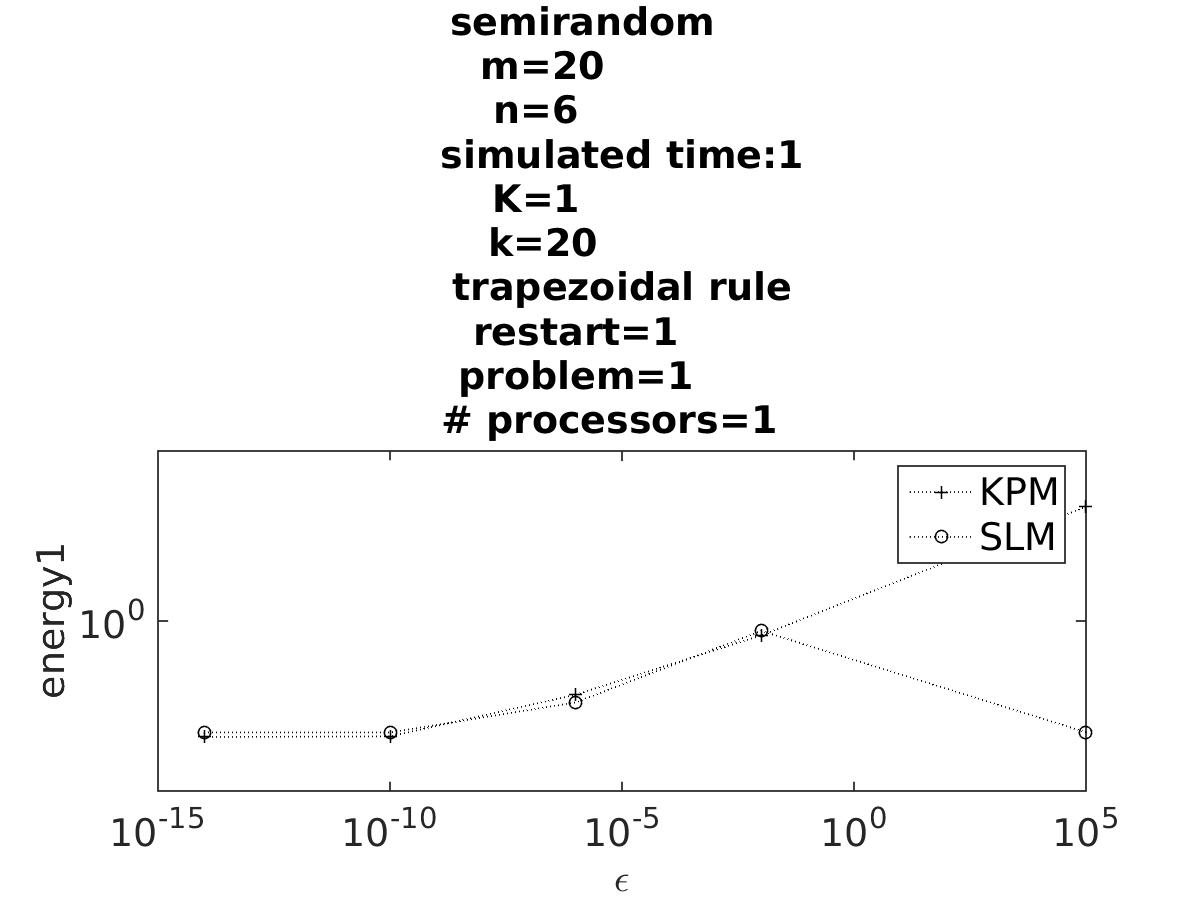
\includegraphics[scale = 0.17]{../MATLAB/fig/compareEnergy.jpg}
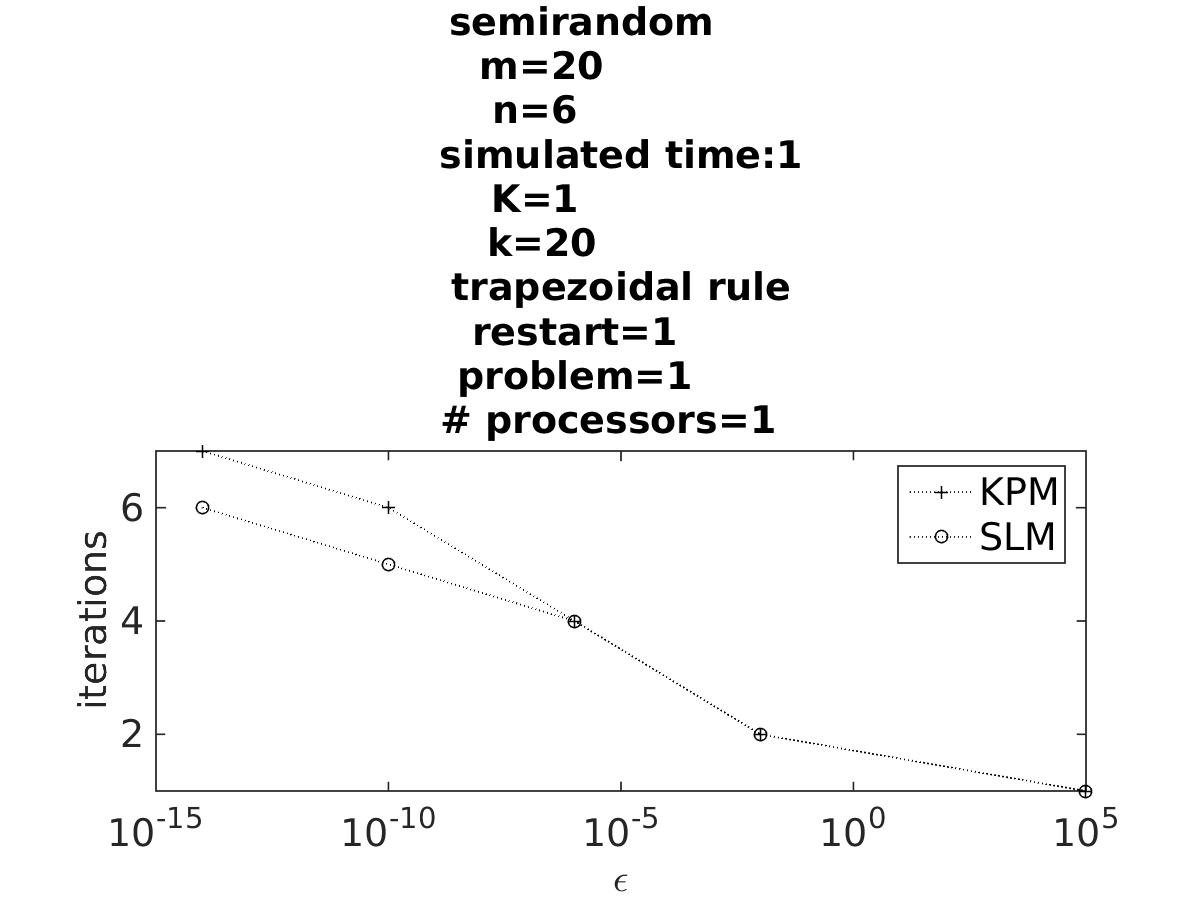
\includegraphics[scale = 0.17]{../MATLAB/fig/compareIter.jpg}
%\caption{Caption}
%\label{fig:my_label}
%\end{figure}

The figures above implies that restarting the symplectic Lanzcos method does not change the energy. But for Arnoldi it changes quite a bit.
To be completely sure that this is what happens, we are going to do everything a bit more precise.

The residual energy of the symplectic Lanzcos method is
$$ \frac{1}{2} e_r^{\top} J A e_r + e_r^\top J r_{n+1} e_{2n}^\top z $$
with $ e_r = y-y_n $ (analytical solution minus approximated solution) and $r_{n+1}$ is given by the symplectic lanzcos method. 






%%%%%%%%%%%%%%%%%%%%%%%%%%%%%%%%%%%%%%%%%%%%%%%%%%%%%%%%%%%%%%%%%%%%%%%%%%%%%%%%%%%%%%%%%%%%%%%%%%%%%%%%%%%%%%%
\chapter{Some results and explanation}
%%%%%%%%%%%%%%%%%%%%%%%%%%%%%%%%%%%%%%%%%%%%%%%%%%%%%%%%%%%%%%%%%%%%%%%%%%%%%%%%%%%%%%%%%%%%%%%%%%%%%%%%%%%%%%%
We will now show some numerical experiments using a randomly generated Hamiltonian matrix(\texttt{semirandom}).
